% Based on a script by Stefano Rosatti
% author: Lukasz Kidzinski
% email: lukasz.kidzinski@stanford.edu
% Stanford University
% August 2016

% #########################################

\documentclass[aspectratio=169]{beamer}
\setbeamertemplate{section in toc}[sections numbered]
\setbeamertemplate{subsection in toc}[subsections numbered]
\setbeamertemplate{caption}{\raggedright\insertcaption\par}
\setbeamertemplate{navigation symbols}{}%remove navigation symbols

\addtobeamertemplate{navigation symbols}{}{%
    \usebeamerfont{footline}%
    \usebeamercolor[fg]{footline}%
    \hspace{1em}%
    \ifnum \theframenumber=1
        % This is the title frame, do nothing

    \else
        % These would be all the following frames
        % <<<Your template code goes here>>>
    {\large \insertframenumber/\inserttotalframenumber}
    \fi
}

   
  
\usepackage{textpos}
\usepackage{graphicx}

\usepackage{fontspec}
\defaultfontfeatures{Ligatures={TeX}}
\setmainfont[HyphenChar={-},ItalicFont=PTF56F.ttf,BoldFont=PTF75F.ttf,BoldItalicFont=PTF76F.ttf]{PTF55F.ttf}
\setsansfont[HyphenChar={-},ItalicFont=PTS56F.ttf,BoldFont=PTS75F.ttf,BoldItalicFont=PTS76F.ttf]{PTS55F.ttf}
\setmonofont[Mapping=tex-text]{Ubuntu Mono}


%% В XeLaTex заменой известного пакета babel является пакет polyglossia.
%% Теперь у нас будут переносы слов
\usepackage{csquotes}
\usepackage{polyglossia}
\setdefaultlanguage{russian}
\setotherlanguage{english}

\usepackage[normalem]{ulem}

\newcommand{\emphnext}[1]{\only<1>{#1}\only<2>{{\color{red} #1}}}
\newcommand{\highlight}[1]{\colorbox{red!30}{#1}}
\newcommand{\highlightnext}[1]{\only<1>{#1}\only<2>\highlight{#1}}


\usetheme{default}
\author[ok.john.rus@gmail.com]{Ori Lahav, \textbf{Egor Namakonov}, Anton Podkopaev, Jonas Oberhauser, Viktor Vafeiadis}
\title[-----]{Making Weak Memory Models Fair}
\institute{
  % \vspace{0.5cm}
  
\raisebox{-1.5cm}{  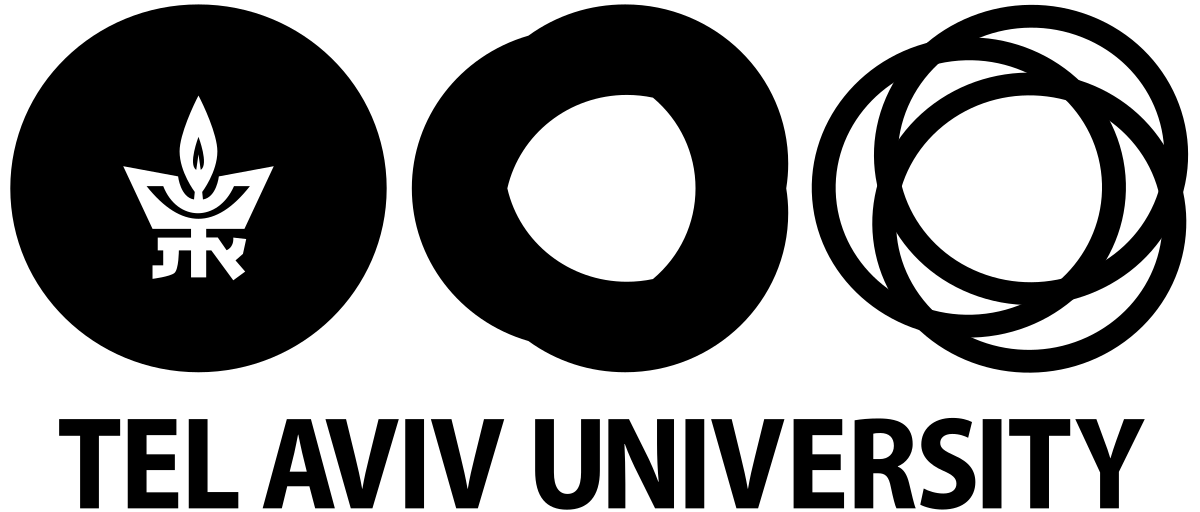
\includegraphics[height=1.0cm]{logos/TelAvivUni_logo}
  \hspace{0.5cm}
  \hfill
  
\includegraphics[height=0.9cm]{logos/spbu_logo}
  \hspace{0.5cm}
  \hfill
  
\includegraphics[height=1.3cm]{logos/jbr_logo}
  \hspace{0.5cm}
  \hfill
  
\includegraphics[height=0.9cm]{logos/huawei_logo}
  \hspace{0.5cm}
  \hfill
  
\includegraphics[height=1.4cm]{logos/hse_logo}
}

  \vspace{0.5cm}  
  
\includegraphics[height=0.6cm]{logos/mpisws_logo}
}
% \AtBeginSection[]
% {
%   \begin{frame}<beamer>
%     \frametitle{Содержание}
%     \tableofcontents[currentsection]
%   \end{frame}
% }

\newcommand{\todo}[1]{{\color{red}\textbf{#1}}}
\graphicspath{ {./} }

\usepackage{booktabs}
\usepackage{siunitx}
%\usepackage{subcaption}
\usepackage{microtype}
\usepackage{amsmath}
\usepackage{amssymb,amsfonts}
\usepackage{stmaryrd}
\usepackage{thm-restate}
\usepackage{multicol}
\usepackage{color}
\usepackage{algorithm}
\usepackage{environ}
\usepackage{float}
\usepackage{multirow}
\usepackage[noend]{algpseudocode}
\usepackage{graphicx}
\usepackage{tikz}
\usepackage{thm-restate}
\usepackage{mathpartir}
\usepackage{xspace}
\usepackage{paralist}
% \usepackage[inline]{enumitem}
\usepackage[capitalize]{cleveref}
\usetikzlibrary{fadings,decorations.pathmorphing,decorations.pathreplacing,shapes}
\usetikzlibrary{calc}
\usetikzlibrary{arrows,automata,arrows.meta}
\usetikzlibrary{positioning}
\usetikzlibrary{spy}
\usepackage{ifthen}
\usepackage{xargs}
\usepackage{pdftexcmds}
% \usepackage{transparent}
\usepackage[nomessages]{fp}
\usepackage{colortbl}

% for setorder
\usepackage{etoolbox}
\usepackage{xstring}


\usepackage{xfp}

\theoremstyle{acmdefinition}
\newtheorem{remark}{Remark}

% enviorments
\AtEndPreamble{%
\theoremstyle{acmplain}
\newtheorem{notation}[theorem]{Notation}
\newtheorem*{notation*}{Notation}
}

% \ifhideproofs

% % Allocate a block of 1000 token registers
% \toks1000={}
% \newcounter{proofcount}

% \NewEnviron{toappendix}{%
%   \global\toks\numexpr\the\toks1000+\value{proofcount}\relax=\expandafter{\BODY}
%   \stepcounter{proofcount}}

% \NewEnviron{proofof}[1]{%
%   \edef\next{%
%     \noexpand\begin{proof}[Proof of \noexpand\cref{\unexpanded\expandafter{#1}}]%
%     \unexpanded\expandafter{\BODY}}%
%   \global\toks\numexpr\the\toks1000+\value{proofcount}\relax=\expandafter{\next\end{proof}}
%   \stepcounter{proofcount}}

% % \printproofs simply loops over the used token registers of the
% % block, freeing their contents
% \makeatletter
% \def\printproofs{%
%   \count@=\z@
%   \loop
%     \the\toks\numexpr\the\toks1000+\count@\relax
%     \ifnum\count@<\value{proofcount}%
%     \advance\count@\@ne
%   \repeat}
% \makeatother

% \else %hideproofs

\NewEnviron{toappendix}{}
\NewEnviron{proofof}[1]{\begin{proof}\BODY\end{proof}}
\newcommand\printproofs{}

% \fi %hideproofs

\crefformat{section}{#2\S{}#1#3}
\Crefname{section}{Section}{Section}
\Crefformat{section}{Section #2#1#3}
\Crefname{figure}{\text{Figure}}{\text{Figures}}
\crefname{corollary}{\text{Corollary}}{\text{corollaries}}
\Crefname{corollary}{\text{Corollary}}{\text{Corollaries}}
\crefname{lemma}{\text{Lemma}}{\text{Lemmas}}
\Crefname{lemma}{\text{Lemma}}{\text{Lemmas}}
\crefname{proposition}{\text{Prop.}}{\text{Propositions}}
\Crefname{proposition}{\text{Proposition}}{\text{Propositions}}
\crefname{definition}{\text{Def.}}{\text{Definitions}}
\Crefname{definition}{\text{Definition}}{\text{Definitions}}
\crefname{notation}{\text{Notation}}{\text{Notations}}
\Crefname{notation}{\text{Notation}}{\text{Notations}}
\crefname{theorem}{\text{Theorem}}{\text{Theorems}}
\Crefname{theorem}{\text{Theorem}}{\text{Theorems}}
\crefname{figure}{\text{Fig.}}{\text{Figures}}
\Crefname{figure}{\text{Figure}}{\text{Figures}}

\newcommand{\citeapp}[1]{\cite[\cref{#1}]{appendix}}

\makeatletter
\newenvironment{claimproof}[1][\proofname]{
  \renewcommand{\qedsymbol}{$\triangleleft$}%
\par
  \pushQED{\qed}%
  \normalfont \topsep6\p@\@plus6\p@\relax
  \list{}{\leftmargin=1.5em
          \rightmargin=0em
          \settowidth{\itemindent}{\itshape#1}%
          \labelwidth=\itemindent
          % the following line is not needed with amsart, but might be with other classes
          \parsep=0pt \listparindent=\parindent 
  }
  \item[\hskip\labelsep
        \itshape
    #1\@addpunct{.}]\ignorespaces
}{%
  \popQED\endlist\@endpefalse
}
\makeatother

\AtEndPreamble{%
\newcounter{claimcounter}
\numberwithin{claimcounter}{theorem}
\newenvironment{claim}[1]{ \refstepcounter{claimcounter}\par\noindent\underline{Claim \theclaimcounter:}\space#1}{}
%\newenvironment{claimproof}[1][\proofname]{%
%  \renewcommand{\qedsymbol}{$\triangleleft$}%
%  \begin{proof}[#1]%
%}{%
%  \end{proof}%
%}

\crefname{claimcounter}{\text{Claim}}{\text{Claims}}
\Crefname{claimcounter}{\text{Claim}}{\text{Claims}}
}

% \let\originalparagraph\paragraph
% \renewcommand{\paragraph}[1]{\originalparagraph{\textbf{#1}}}

\newcommand{\textdom}[1]{\mathsf{#1}}
\newcommand{\textcode}[1]{\texorpdfstring{\texttt{#1}}{#1}}
\newcommand{\kw}[1]{\textbf{\textcode{#1}}}
\newcommand{\skipc}{\kw{skip}}
\newcommand{\ite}[3]{\kw{if}\;#1\:\kw{then}\;#2\;\\ \kw{else}\;#3}
\newcommand{\itesl}[3]{\kw{if}\;#1\:\kw{then}\;#2\;\kw{else}\;#3}
\newcommand{\iteml}[3]{
  \kw{if} \; #1\\
  \begin{array}[t]{@{}l@{}l}
    \kw{then}& \begin{array}[t]{l} #2 \end{array} \\
    \kw{else}& \begin{array}[t]{l} #3 \end{array} \\
  \end{array}
}
\newcommand{\itne}[2]{\kw{if}\;#1\:\kw{then}\\ \quad\;{#2}}
\newcommand{\letdef}[2]{\kw{let}\;#1\;\defeq\;#2\;\kw{in}}

\newcommand{\ALT}{\;\;|\;\;}
\newcommand{\ie}{\emph{i.e.,} }
\newcommand{\eg}{\emph{e.g.,} }
\newcommand{\etal}{\emph{et~al.}}
\newcommand{\wrt}{w.r.t.~}
\newcommand{\aka}{a.k.a.~}

\newcommand{\inarrT}[1]{\begin{array}[t]{@{}l@{}}#1\end{array}}
\newcommand{\inarrC}[1]{\begin{array}{@{}c@{}}#1\end{array}}
\newcommand{\inpar}[1]{\left(\begin{array}{@{}l@{}}#1\end{array}\right)}
\newcommand{\inset}[1]{\left\{\begin{array}{@{}l@{}}#1\end{array}\right\}}
\newcommand{\inarr}[1]{\begin{array}{@{}l@{}}#1\end{array}}
\newcommand{\inarrII}[2]{\begin{array}{@{}l@{~~}||@{~~}l@{}}\inarr{#1}&\inarr{#2}\end{array}}
\newcommand{\inarrIII}[3]{\begin{array}{@{}l@{~~}||@{~~}l@{~~}||@{~~}l@{}}\inarr{#1}&\inarr{#2}&\inarr{#3}\end{array}}
\newcommand{\inarrIV}[4]{\begin{array}{@{}l@{~~}||@{~~}l@{~~}||@{~~}l@{~~}||@{~~}l@{}}\inarr{#1}&\inarr{#2}&\inarr{#3}&\inarr{#4}\end{array}}
\newcommand{\inarrV}[5]{\begin{array}{@{}l@{~~}||@{~~}l@{~~}||@{~~}l@{~~}||@{~~}l@{~~}||@{~~}l@{}}\inarr{#1}&\inarr{#2}&\inarr{#3}&\inarr{#4}&\inarr{#5}\end{array}}

% \renewcommand{\comment}[1]{\color{teal}{~~\texttt{/\!\!/}\textit{#1}}}
\newcommand{\comment}[1]{\color{teal}{\texttt{/\!\!/}\textit{#1}}}
\newcommand{\nocomment}[1]{\color{red!80!black}{~~\texttt{/\!\!/}\textit{#1}}}


\newcommand{\set}[1]{\{{#1}\}}
\newcommand{\sem}[1]{\llbracket #1 \rrbracket}
\newcommand{\pfn}{\rightharpoonup}
\newcommand{\fpfn}{\mathrel{\stackrel{\mathsf{fin}}{\rightharpoonup}}}
\newcommand{\st}{\; | \;}
\newcommand{\N}{{\mathbb{N}}}
\newcommand{\dom}[1]{\textit{dom}{({#1})}}
\newcommand{\codom}[1]{\textit{codom}{({#1})}}
\newcommand{\before}[2]{{#1}_{#2}^\uparrow}
\newcommand{\after}[2]{{#1}_{#2}^\downarrow}
%\newcommand{\fv}[1]{fv{[{#1}]}}
\newcommand{\tup}[1]{{\langle{#1}\rangle}}
\newcommand{\nin}{\not\in}
\newcommand{\suq}{\subseteq}
\newcommand{\sqsuq}{\sqsubseteq}
\newcommand{\sqsu}{\sqsubset}
\newcommand{\sqslq}{\sqsupseteq}
\newcommand{\size}[1]{|{#1}|}
% \newcommand{\block}[1]{\langle {#1}\rangle}
\newcommand{\true}{\top}

\newcommand{\maketil}[1]{{#1}\ldots{#1}}
\newcommand{\til}{\maketil{,}}
\newcommand{\cuptil}{\maketil{\cup}}
\newcommand{\uplustil}{\maketil{\uplus}}
\newcommand{\plustil}{\maketil{+}}
\newcommand{\timestil}{\maketil{\times}}
\newcommand{\paralleltil}{\maketil{\parallel}}
\newcommand{\cdottil}{\maketil{\cdot}}

\renewcommand*{\mathellipsis}{\mathinner{{\ldotp}{\ldotp}{\ldotp}}}
\newcommand{\rst}[1]{|_{#1}}
\newcommand{\imm}[1]{{#1}{\rst{\text{imm}}}}
\renewcommand{\succ}[2]{\text{succ}_{#1}(#2)}
\newcommand{\aite}[3]{(#1\;?\;#2:#3)}
%\newcommand{\defeq}{\mathrel{\stackrel{\mathsf{def}}{=}}}
\newcommand{\defiff}{\mathrel{\stackrel{\mathsf{\triangle}}{\Leftrightarrow}}}
\newcommand{\defeq}{\triangleq}
\newcommand{\powerset}[1]{\mathcal{P}({#1})}
\newcommand{\finpowerset}[1]{\mathcal{P}_{<\omega}({#1})}
%\renewcommand{\implies}{\Rightarrow}

\makeatletter
\newcommand{\raisemath}[1]{\mathpalette{\raisem@th{#1}}}
\newcommand{\raisem@th}[3]{\raisebox{#1}{$#2#3$}}
\makeatother

\newcommandx{\yaHelper}[2][1=\empty]{%
\ifthenelse{\equal{#1}{\empty}}%
  { \ensuremath{ \scriptstyle{ #2 } } } % no offset
  { \raisebox{ #1 }[0pt][0pt]{ \ensuremath{ \scriptstyle{ #2 } } } }  % with offset
}

\newcommandx{\yrightarrow}[4][1=\empty, 2=\empty, 4=\empty, usedefault=@]{%
  \ifthenelse{\equal{#2}{\empty}}
  { \xrightarrow{ \protect{ \yaHelper[ #4 ]{ #3 } } } } % there's no text below
  { \xrightarrow[ \protect{ \yaHelper[ #2 ]{ #1 } } ]{ \protect{ \yaHelper[ #4 ]{ #3 } } } } % there's text below
}

\newcommand{\astep}[1]{
\ifthenelse{\equal{#1}{\empty}}{\xrightarrow{}}
{\mathrel{\raisebox{-0.8pt}{\ensuremath{\xrightarrow{#1}}}}}}
\newcommand{\bstep}[1]{\xRightarrow{#1}}
\newcommand{\tcstep}[1]{\astep{#1}^{\raisemath{-2pt}{*}}}

\colorlet{colorPO}{gray!60!black}
\colorlet{colorRF}{green!60!black}
\colorlet{colorMO}{orange}
\colorlet{colorFR}{purple}
\colorlet{colorECO}{red!80!black}
\colorlet{colorSYN}{green!40!black}
\colorlet{colorHB}{blue}
\colorlet{colorPPO}{magenta}
\colorlet{colorPB}{olive}
\colorlet{colorSBRF}{olive}
\colorlet{colorRMW}{olive!70!black}
\colorlet{colorRSEQ}{blue}
\colorlet{colorSC}{violet}
\colorlet{colorPSC}{violet}
\colorlet{colorREL}{olive}
\colorlet{colorCONFLICT}{olive}
\colorlet{colorRACE}{olive}
\colorlet{colorWB}{orange!70!black}
\colorlet{colorPSC}{violet}
\colorlet{colorSCB}{violet}
\colorlet{colorDEPS}{violet}
\colorlet{colorBF}{green!40!black}

\tikzset{
   % every path/.style={>=stealth},
   po/.style={->,color=colorPO,thin,shorten >=-0.5mm,shorten <=-0.5mm},
   sw/.style={->,color=colorSYN,shorten >=-0.5mm,shorten <=-0.5mm},
   rf/.style={->,color=colorRF,dashed,,shorten >=-0.5mm,shorten <=-0.5mm},
   hb/.style={->,color=colorHB,thick,shorten >=-0.5mm,shorten <=-0.5mm},
   mo/.style={->,color=colorMO,dotted,very thick,shorten >=-0.5mm,shorten <=-0.5mm},
   wb/.style={->,color=colorMO,dotted,very thick,shorten >=-0.5mm,shorten <=-0.5mm},
   no/.style={->,dotted,thick,shorten >=-0.5mm,shorten <=-0.5mm},
   fr/.style={->,color=colorFR,dotted,thick,shorten >=-0.5mm,shorten <=-0.5mm},
   deps/.style={->,color=colorDEPS,dotted,thick,shorten >=-0.5mm,shorten <=-0.5mm},
   rmw/.style={->,color=colorRMW,thick,shorten >=-0.5mm,shorten <=-0.5mm},
   % mem/.style={-to,color=colorPO,thick,},
   mem/.style={-Latex,color=colorPO,thick,},
   time/.style={-to,dashed,color=colorPO,thick},
   frComp/.style={->,color=colorFR,line width=3,opacity=0.5},
   thicc/.style={->,color=gray,thick,line width=5,opacity=1},
   prop/.style={-,color=gray,shorten >=0.0cm,shorten <=0.2cm},
}

%% Orders
\newcommand{\na}{\mathtt{na}}
\newcommand{\pln}{\mathtt{pln}}
\newcommand{\rlx}{\mathtt{rlx}}
\newcommand{\rel}{{\mathtt{rel}}}
\newcommand{\acq}{{\mathtt{acq}}}
\newcommand{\acqrel}{{\mathtt{acqrel}}}
\newcommand{\sco}{{\mathtt{sc}}}
\newcommand{\sto}{{\mathtt{st}}}
\newcommand{\full}{{\mathtt{sy}}}
\newcommand{\ld}{{\mathtt{ld}}}
\newcommand{\isb}{{\mathtt{isb}}}

%% Event labels

\newcommand{\evlab}[4]{{#1}^{#2}({#3},{#4})}
\newcommand{\evflab}[1]{{\lF}^{#1}}
\newcommand{\evulab}[4]{{\lU}^{#1}({#2},{#3},{#4})}
\newcommand{\rlab}[3]{{\lR}^{#1}({#2},{#3})}
\newcommand{\erlab}[4]{{\lR}^{#1}({#2},{#3},{#4})}
\newcommand{\wlab}[3]{{\lW}^{#1}({#2},{#3})}
\newcommand{\flab}[1]{{\lF}^{#1}}
\newcommand{\ulab}[4]{{\lU}^{#1}({#2},{#3},{#4})}
\newcommand{\slab}{{\lS}}
\newcommand{\proplab}{{\mathtt{prop}}}

\newcommand{\lE}{{\mathtt{E}}}
\newcommand{\lC}{{\mathtt{C}}}
%\newcommand{\lP}{{\mathit{P}}}
\newcommand{\lM}{{\mathtt{M}}}
\newcommand{\lS}{{\mathtt{Skip}}}
\newcommand{\lR}{{\mathtt{R}}}
\newcommand{\lW}{{\mathtt{W}}}
\newcommand{\lA}{{\mathtt{A}}}
\newcommand{\lQ}{{\mathtt{Q}}}
\newcommand{\lL}{{\mathtt{L}}}
\newcommand{\lU}{{\mathtt{U}}}
\newcommand{\lF}{{\mathtt{F}}}
\newcommand{\lRES}{{\mathtt{Res}}}
\newcommand{\lAT}{{\mathtt{At}}}
\newcommand{\lATR}{{\mathtt{AtR}}}
\newcommand{\linit}{{\mathtt{init}}}
\newcommand{\lSigma}{{\mathbf{\Sigma}}}
\newcommand{\lTheta}{{\mathbf{\Theta}}}

\newcommand{\lTLAB}{{\mathtt{tlab}}}
\newcommand{\lLAB}{{\mathtt{elab}}}
\newcommand{\lTID}{{\mathtt{tid}}}
\newcommand{\lSN}{{\mathtt{sn}}}
\newcommand{\lTYP}{{\mathtt{typ}}}
\newcommand{\lLOC}{{\mathtt{loc}}}
\newcommand{\lMOD}{{\mathtt{mod}}}
\newcommand{\lXMOD}{{\mathtt{xmod}}}
\newcommand{\lRMWST}{{\mathtt{rmwst}}}
\newcommand{\lVALR}{{\mathtt{val_r}}}
\newcommand{\lVALW}{{\mathtt{val_w}}}
\newcommand{\lELAB}{{\mathtt{elab}}}
\newcommand{\lAVALS}{{\mathtt{atvals}}}

\newcommand{\lSRC}{{\mathtt{src}}}
\newcommand{\lTGT}{{\mathtt{tgt}}}

\newcommand{\lTS}{{\mathtt{ts}}}
\newcommand{\lVIEW}{{\mathtt{view}}}
\newcommand{\lVAL}{{\mathtt{val}}}


\newcommand{\lSTART}{{\mathtt{k}}}
\newcommand{\lLENGTH}{{\mathtt{n}}}

%% Relations

\newcommand{\po}{{\color{colorPO}\mathit{po}}}
\newcommand{\rf}{{\color{colorRF}\mathit{rf}}}
\newcommand{\mo}{{\color{colorMO}\mathit{mo}}}
\newcommand{\hb}{{\color{colorHB}\mathit{hb}}}
\newcommand{\rb}{{\color{colorFR}\mathit{rb}}}
\newcommand{\wmo}{{\color{colorMO}\mathit{wmo}}}
\newcommand{\wrb}{{\color{colorFR}\mathit{wrb}}}
\newcommand{\fo}{{\color{colorECO}\mathtt{fo}}}

\newcommand{\lX}{\mathtt{X}}
\newcommand{\lPO}{{\color{colorPO}\mathtt{po}}}
\newcommand{\lRF}{{\color{colorRF} \mathtt{rf}}}
\newcommand{\lRMW}{{\color{colorRMW} \mathtt{rmw}}}
\newcommand{\lMO}{{\color{colorMO} \mathtt{mo}}}
\newcommand{\lMOx}{{\color{colorMO} \mathtt{mo}}_x}
\newcommand{\lMOy}{{\color{colorMO} \mathtt{mo}}_y}
\newcommand{\lCO}{{\color{colorMO} \mathtt{co}}}
\newcommand{\lCOx}{{\color{colorMO} \mathtt{co}}_x}
\newcommand{\lCOy}{{\color{colorMO} \mathtt{co}}_y}
\newcommand{\lFR}{{\color{colorFR} \mathtt{rb}}}
\newcommand{\lFRx}{{\color{colorFR} \mathtt{fr}}_x}
\newcommand{\lFRy}{{\color{colorFR} \mathtt{fr}}_y}
\newcommand{\lECO}{{\color{colorECO} \mathtt{eco}}}
\newcommand{\lSBRF}{{\color{colorSBRF} \mathtt{sbrf}}}
\newcommand{\lRSEQ}{{\color{colorRSEQ}\mathtt{rseq}}}
\newcommand{\lSW}{{\color{colorSYN}\mathtt{sw}}}
\newcommand{\lHB}{{\color{colorHB}\mathtt{hb}}}
\newcommand{\lHBSC}{{\color{colorHB}\mathtt{hb}}_{\SC}}
\newcommand{\lHBTSO}{{\color{colorHB}\mathtt{hb}}_{\TSO}}
\newcommand{\lHBRA}{{\color{colorHB}\mathtt{hb}}_{\RA}}
\newcommand{\lPORF}{{\lPO\lRF}}
%\newcommand{\lWB}{{\color{colorWB} \mathtt{wb}}}
\newcommand{\lDOB}{{\mathtt{dob}}}
\newcommand{\lBOB}{{\mathtt{bob}}}
\newcommand{\lAOB}{{\mathtt{aob}}}
\newcommand{\lOBS}{{\mathtt{obs}}}
\newcommand{\lEORD}{{\mathtt{eord}}}
\newcommand{\lTORD}{{\mathtt{tord}}}
\newcommand{\lPPO}{{\color{colorPPO}\mathtt{ppo}}}
\newcommand{\lBF}{{\color{colorBF}\mathtt{bf}}}
\newcommand{\rpo}{\widehat{\lPO}}

\newcommand{\lSC}{{\mathtt{sc}}}
\newcommand{\lRA}{{\mathtt{ra}}}

\newcommand{\lSCB}{{\color{colorSCB} \mathtt{scb}}}
\newcommand{\lPSC}{{\color{colorPSC} \mathtt{psc}}}
\newcommand{\lPSCB}{\lPSC_{\rm base}}
\newcommand{\lPSCF}{\lPSC_\lF}
\newcommand{\lCONFLICT}{{\color{colorCONFLICT} \mathtt{conflict}}}
\newcommand{\lRACE}{{\color{colorRACE} \mathtt{race}}}
\newcommand{\lNARACE}{{\color{colorRACE} \mathtt{na-race}}}

\newcommand{\lmakeW}[1]{\mathtt{w}#1}
\newcommand{\lWFR}{\lmakeW{\lFR}}
\newcommand{\lWECO}{\lmakeW{\lECO}}
\newcommand{\lWSCB}{\lmakeW{\lSCB}}
\newcommand{\lWPSCB}{\lmakeW{\lPSCB}}
\newcommand{\lWPSCF}{\lmakeW{\lPSCF}}
\newcommand{\lWPSC}{\lmakeW{\lPSC}}
\newcommand{\lWB}{\lmakeW{\lMO}}

\newcommand{\lDEPS}{{{\color{colorDEPS}\mathtt{deps}}}}
\newcommand{\lCTRL}{{{\color{colorDEPS}\mathtt{ctrl}}}}
\newcommand{\lCTRLISYNC}{{{\color{colorDEPS}\mathtt{ctrl_{isync}}}}}
\newcommand{\lDATA}{{{\color{colorDEPS}\mathtt{data}}}}
\newcommand{\lADDR}{{{\color{colorDEPS}\mathtt{addr}}}}

\newcommand{\lmakeE}[1]{#1\mathtt{e}}
\newcommand{\lRFE}{\lmakeE{\lRF}}
\newcommand{\lCOE}{\lmakeE{\lCO}}
\newcommand{\lFRE}{\lmakeE{\lFR}}
\newcommand{\lMOE}{\lmakeE{\lMO}}
\newcommand{\lmakeI}[1]{#1\mathtt{i}}
\newcommand{\lRFI}{\lmakeI{\lRF}}
\newcommand{\lCOI}{\lmakeI{\lCO}}
\newcommand{\lFRI}{\lmakeI{\lFR}}

\newcommand{\dpo}[2]{\draw[po] (#1) edge (#2);}
\newcommand{\dpoText}[2]{\draw[po] (#1) edge[right] node {$\lPO$} (#2);}
% \newcommand{\dfr}[3]{\draw[fr] (#1) edge[#3] node {$\lFR$} (#2);}
\newcommandx{\dfr}[5][3={},4={},5={}]{\draw[fr,#3] (#1) edge[#5] node[#4] {$\lFR$} (#2);}
% \newcommand{\drf}[3][]{\draw[rf, #1] (#2) edge node[right] {$\lRF$} (#3);}
\newcommandx{\drf}[4][3={},4={}]{\draw[rf, #3] (#1) edge node[right,#4] {$\lRF$} (#2);}

% \newcommand{\dmo}[2]{\draw[mo] (#1) edge node {$\lMO$} (#2);}
\newcommand{\dmoext}[3]{\draw[mo, #3] (#1) edge node {$\lMO$} (#2);}
\newcommandx{\dmo}[4][1=, 2=right]{\draw[mo, #1] (#3) edge node[#2] {$\lMO$} (#4);}
% \newcommandx{\d}[4][1=, 2=right]{\draw[mo, #1] (#3) edge node[#2] {$\lMO$} (#4);}

\newcommand{\Event}{\mathsf{Event}}
\newcommand{\Init}{\mathsf{Init}}
\newcommand{\Tid}{\mathsf{Tid}}
\newcommand{\Loc}{\mathsf{Loc}}
\newcommand{\Val}{\mathsf{Val}}
\newcommand{\Lab}{\mathsf{ELab}}
\newcommand{\Mod}{\mathsf{Mod}}
\newcommand{\Modr}{\mathsf{Mod}_{\lR}}
\newcommand{\Modw}{\mathsf{Mod}_{\lW}}
\newcommand{\Modf}{\mathsf{Mod}_{\lF}}
\newcommand{\Modrmw}{\mathsf{Mod}_{\lU}}
\newcommand{\Exec}{\mathsf{EGraph}}
\newcommand{\SProg}{\mathsf{SProg}}
\newcommand{\Inst}{\mathsf{Inst}}
\newcommand{\Exp}{\mathsf{Exp}}
\newcommand{\Reg}{\mathsf{Reg}}


\newcommand{\readInst }[2]{#1 \;{:=}\;[\,#2\,]}
\newcommand{\fenceInst}{\kw{fence}}
\newcommand{\ifGotoInst}[2]{\kw{if} \; #1 \; \kw{goto} \; #2}
\newcommand{\gotoInst}[1]{\kw{goto} \; #1}
\newcommand{\writeInst}[2]{[\,#1\,]\;{:=}\;#2}
\newcommand{\assignInst}[2]{#1\;{:=}\;#2}
\newcommand{\incInstP}[2]{\faddInstn({#1},{#2})}
\newcommand{\incInst}[3]{#1 \;{:=}\;\faddInstn({#2},{#3})}
\newcommand{\casInst}[4]{#1 \;{:=}\;\casInstn({#2},{#3} \shortrightarrow {#4})}
\newcommand{\waitInst}[2]{\kw{wait}({#1} = {#2})}
\newcommand{\casInstn}{\kw{CAS}}
\newcommand{\faddInstn}{\kw{FADD}}
\newcommand{\funcDecl}[4]{
    #1 \; #2(#3) \; \{ \;
    \begin{array}[t]{@{}l@{}}
    \\ #4
    \; \}
    \end{array}  \\
}
\newcommand{\funcDeclsl}[4]{
    #1 \; #2(#3) \; \{ \; #4 \; \}
}

% \newcommand{\repeatInst}[2]{\kw{repeat}\; \{\; #1 \;\}\;\kw{until}\;#2}
\newcommand{\repeatInst}[2]{\kw{repeat}\;  #1 \;\kw{until}\;#2}

\newcommand{\while}[2]{\kw{while}\;#1\;\{\; #2 \; \}}
\newcommand{\whileml}[2]{
\kw{while} \; #1 \; \{ \\
\quad
\begin{array}{@{}l@{}}
#2
\end{array} \\
\}
}
\newcommand{\repeatml}[2]{
\kw{repeat} \; \{ \;
\begin{array}[t]{@{}l@{}}
#1 \; \}
\end{array} \\
%% \phantom{\kw{repeat} \; \}} \;
\quad \kw{until} \, #2
}
\newcommand{\classDecl}[2]{
    \kw{class} \; #1 \; \{ \\
    \quad
    \begin{array}{@{}l l@{}}
    #2
    \end{array} \\
    \} \\
}

% Models

\newcommand{\RC}{\ensuremath{\mathsf{RC11}}\xspace}
\newcommand{\WRC}{\ensuremath{\mathsf{WRC11}}\xspace}

\newcommand{\SC}{\ensuremath{\mathsf{SC}}\xspace}
\newcommand{\SCopfair}{\ensuremath{\mathsf{SC^{fair}_{op}}}\xspace}
\newcommand{\SCdecl}{\ensuremath{\mathsf{SC_{decl}}}\xspace}
\newcommand{\SCdeclfair}{\ensuremath{\mathsf{SC^{fair}_{decl}}}\xspace}

\newcommand{\TSO}{\ensuremath{\mathsf{TSO}}\xspace}
\newcommand{\TSOopfair}{\ensuremath{\mathsf{TSO^{fair}_{op}}}\xspace}
\newcommand{\TSOdecl}{\ensuremath{\mathsf{TSO_{decl}}}\xspace}
\newcommand{\TSOdeclfair}{\ensuremath{\mathsf{TSO^{fair}_{decl}}}\xspace}

\newcommand{\RA}{\ensuremath{\mathsf{RA}}\xspace}
\newcommand{\RAopfair}{\ensuremath{\mathsf{RA^{fair}_{op}}}\xspace}
\newcommand{\RAdecl}{\ensuremath{\mathsf{RA_{decl}}}\xspace}
\newcommand{\RAdeclfair}{\ensuremath{\mathsf{RA^{fair}_{decl}}}\xspace}

\newcommand{\SCOH}{\ensuremath{\mathsf{StrongCOH}}\xspace}
\newcommand{\SCOHopfair}{\ensuremath{\mathsf{StrongCOH^{fair}_{op}}}\xspace}
\newcommand{\SCOHdecl}{\ensuremath{\mathsf{StrongCOH_{decl}}}\xspace}
\newcommand{\SCOHdeclfair}{\ensuremath{\mathsf{StrongCOH^{fair}_{decl}}}\xspace}

\newcommand{\fairDecl}{\ensuremath{\mathsf{Fair_{decl}}}\xspace}

% \newcommand{\ARM}{\ensuremath{\mathsf{ARM}}\xspace}
% \newcommand{\ARMra}{\ensuremath{\mathsf{ARMra}}\xspace}

\newcounter{mylabelcounter}

\makeatletter
\newcommand{\labelAxiom}[2]{%
\hfill{\normalfont\textsc{(#1)}}\refstepcounter{mylabelcounter}
\immediate\write\@auxout{%
  %% \string\newlabel{#2}{{1}{\thepage}{{#1}}{mylabelcounter.\number\value{mylabelcounter}}{}}
  \string\newlabel{#2}{{\unexpanded{\normalfont\textsc{#1}}}{\thepage}{{\unexpanded{\normalfont\textsc{#1}}}}{mylabelcounter.\number\value{mylabelcounter}}{}}
}%
}
\makeatother

\newcommand{\squishlist}[1][$\bullet$]{%[$\tinybullet$]{
 \begin{list}{#1}
  { \setlength{\itemsep}{0pt}
     \setlength{\parsep}{0pt}
     \setlength{\topsep}{1pt}
     \setlength{\partopsep}{0pt}
     \setlength{\leftmargin}{1.2em}
     \setlength{\labelwidth}{0.5em}
     \setlength{\labelsep}{0.4em} } }
\newcommand{\squishend}{
  \end{list}  }

% \newcommand{\todo}[1]{{\color{blue}\textbf{TODO: #1}}}
\newcommand{\TODO}[1]{\todo{TODO: #1}}
\newcommand{\ori}[1]{{\color{red!70!black}\textbf{ORI: #1}}}
\newcommand{\viktor}[1]{{\color{green!80!black}\textbf{VV: #1}}}
\newcommand{\red}[1]{{\color{red}{#1}}}
\newcommand{\app}[1]{{\color{blue!80!black}\textbf{ANTON: #1}}}
\newcommand{\egor}[1]{{\color{green!60!blue}\textbf{EGOR: #1}}}

\newcommand{\m}{{M}}
\renewcommand{\b}{{B}}
\newcommand{\buff}{{b}}

\newcommand{\A}{{A}}
\newcommand{\init}{\mathit{init}}
\newcommand{\M}{{\mathcal{M}}}
\newcommand{\sys}{{\mathit{CS}}}
\newcommand{\sprog}{S}
\newcommand{\prog}{{P}}
\newcommand{\loc}{{x}}
\newcommand{\loca}{{y}}
\newcommand{\locb}{{z}}
\newcommand{\locc}{{w}}
\newcommand{\locf}{{f}}
\newcommand{\tid}{{\tau}}
\newcommand{\tida}{{\pi}}
\newcommand{\lab}{{l}}
\newcommand{\val}{v}
\newcommand{\valr}{\val_\lR}
\newcommand{\valw}{\val_\lW}

\newcommand{\add}{{\mathsf{add}}}
\newcommand{\pc}{\mathit{pc}}

\newcommand{\thread}[1]{T_#1}

\newcommand{\beh}{\beta}
%\newcommand{\behf}[1]{\mathsf{beh}({#1})}
\newcommand{\Beh}[1]{\mathsf{B}({#1})}
\newcommand{\Behtf}[1]{\mathsf{B^{tf}}({#1})}
\newcommand{\Behmf}[1]{\mathsf{B^{mf}}({#1})}
\newcommand{\Behfin}[1]{\mathsf{B^{fin}}({#1})}

\newcommand{\Traces}[1]{\mathsf{Tr}({#1})}
%\newcommand{\Tracestf}[1]{\mathsf{Tr^{tf}}({#1})}
%\newcommand{\Tracesmf}[1]{\mathsf{Tr^{mf}}({#1})}
\newcommand{\Tracesfin}[1]{\mathsf{Tr^{fin}}({#1})}

\newcommand{\OTraces}[1]{\mathsf{OTr}({#1})}
%\newcommand{\OTracestf}[1]{\mathsf{OTr^{tf}}({#1})}
%\newcommand{\OTracesmf}[1]{\mathsf{OTr^{mf}}({#1})}
\newcommand{\OTracesfin}[1]{\mathsf{OTr^{fin}}({#1})}

\newcommand{\en}{\nu}
\renewcommand{\G}{\mathcal{G}}
\newcommand{\fair}{\texttt{fair}}

% Timestamp machine definitions
\newcommand{\Time}{\mathsf{Time}}
\newcommand{\View}{\mathsf{View}}
\newcommand{\Msg}{\mathsf{Msg}}
\newcommand{\msga}{m}
\newcommand{\msgb}{m'}

\newcommand{\ts}{t}
\newcommand{\msg}[4]{\tup{#1:#2@#3,#4}}
\newcommand{\view}{\mathit{V}}
\newcommand{\viewinit}{\mathtt{V}_{\text{init}}}
\newcommand{\memoryinit}{\mathtt{memory}_{\text{init}}}
\newcommand{\Tview}{\mathit{T}}
\newcommand{\tsa}{\mathit{tsa}}
\newcommand{\Fview}{\mathit{f}}

\newcommand{\ev}[3]{\tup{#1, #2 : #3}}

\newcommand{\progstate}{\overline{p}}
\newcommand{\memstate}{m}
%\newcommand{\cs}[2]{{{#1}\shortparallel{#2}}{}}
\newcommand{\seq}{\mathbin{;}}

%\newcommand{\beh}{\mathtt{beh}}
\newcommand{\run}{\mu}
\newcommand{\trace}{\rho}
\newcommand{\traces}{S}

\newcommand{\toeventsgen}[2]{\overline{#1}^{#2}}
\newcommand{\toevents}[1]{\toeventsgen{\trace}{#1}}
\newcommand{\evorder}{<_{\trace}}
\newcommand{\tstep}[2]{#1 : #2}
\newcommand{\itstep}[3]{#1 : #2 \square #3}
\newcommand{\tmap}{\mathsf{tmap}}
\newcommand{\tmaplift}{\overline{\tmap}}
\newcommand{\smap}{\mathsf{smap}}
\newcommand{\vmap}{\mathsf{vmap}}
\newcommand{\tslot}{\mathsf{tslot}}
\newcommand{\simrel}{{\mathcal{I}}}
\newcommand{\safepoints}{\mathsf{safepoints}}
\newcommand{\proppoint}{\mathsf{proppoint}}
\newcommand{\etom}{\mathsf{e2m}}
\newcommand{\vmapprop}{\mathsf{vmap}_\proplab}
\newcommand{\vmapfull}{\mathsf{vmap}_{\mathsf{full}}}
\newcommand{\settoview}{\mathsf{set2view}}

\newcommand{\mapn}{\mathsf{map}_\mathsf{n}}
\newcommand{\mapf}{\mathsf{map}}

\newcommand{\pushloop}{\mathsf{push\text{-}loop}}
\newcommand{\unsucpush}{\mathsf{unsuc\text{-}push}}
\newcommand{\sucpush}{\mathsf{suc\text{-}push}}

\newcommand{\poploop}{\mathsf{pop\text{-}loop}}
\newcommand{\emptypop}{\mathsf{empty\text{-}pop}}
\newcommand{\unsucpop}{\mathsf{unsuc\text{-}pop}}
\newcommand{\sucpop}{\mathsf{suc\text{-}pop}}

\newcommand{\concat}{\mathsf{concat}}
\newcommand{\concatOp}{%
  \mathbin{{+}\mspace{-6mu}{+}}%
}
\newcommand{\bmgc}{\mathsf{BMGC}}


\newcommand{\lRs}{(\lR \setminus \lU)}
\newcommand{\lWs}{(\lW \setminus \lU)}

\newcommand{\lISB}{\mathtt{F^{\isb}}}
\newcommand{\lDMB}{\mathtt{DMB}}
%% \newcommand{\lDMBFULL}{\mathtt{DMB.full}}
%% \newcommand{\lDMBLD}{\mathtt{DMB.ld}}
%% \newcommand{\lDMBST}{\mathtt{DMB.st}}
\newcommand{\lDMBSY}{\mathtt{F^{\full}}}
\newcommand{\lDMBLD}{\mathtt{F^{\ld}}}
\newcommand{\lDMBST}{\mathtt{F^{\sto}}}
\newcommand{\SY}{\mathtt{SY}}
\newcommand{\LD}{\mathtt{LD}}
\newcommand{\ST}{\mathtt{ST}}

\newcommand{\RMWst}{\mathsf{RMWst}}
\newcommand{\Excl}{\mathsf{Excl}}
\newcommand{\Bool}{\mathsf{Bool}}

\newcommand{\unset}{\mathtt{unset}}
\newcommand{\readBy}[1]{\mathtt{readBy}\;#1}
\newcommand{\updatedBy}[1]{\mathtt{updatedBy}\;#1}

\newcommand{\isex}{{\mathtt{ex}}}
\newcommand{\isnotex}{{\operatorname{\mathtt{not-ex}}}}
\newcommand{\lWex}{\lW^{\isex}}

\newcommand{\xmod}{{xmod}}
\newcommand{\rmwst}{{rmwst}}

\newcommand{\applyBuffer}{\mathsf{apply\text{-}buffer}}
\newcommand{\blockWrite}{\mathsf{block\text{-}write}}
\newcommand{\promoteMessage}{\mathsf{promote\text{-}message}}
\newcommand{\localb}{b}

%%% Local Variables:
%%% mode: latex
%%% TeX-master: "oopsla"
%%% End:


\declaretheorem[name=Theorem.,style=default,numberwithin=section]{thm}
\declaretheorem[name=Lemma.,style=default,numberwithin=section]{lem}
\declaretheorem[name=Definition,style=default,sibling=thm]{mydefinition}

\newcommand{\pic}[2]{
  \begin{center}
    \includegraphics[scale=#2]{#1}
  \end{center}
}
\newcommand{\twocolumns}[4]{
  \begin{columns}
    \begin{column}{#3}
      #1
    \end{column}
    \begin{column}{#4}
      #2
    \end{column}
  \end{columns}
}
\newcommand{\twocolumnsEq}[2]{
  \twocolumns{#1}{#2}{0.5\linewidth}{0.5\linewidth}
}

\newcommand{\colorTitleApprox}{blue!80!black}

% For some reason \implies is drawn incorrectly
\renewcommand{\implies}{\Rightarrow}

%%% Local Variables:
%%% mode: latex
%%% TeX-master: "oopsla"
%%% End:
